\section{Introduction}

En informatique, l'information se code comme une suite de
bits (en général regroupés en octets). Sur le disque dur, cette information est répartie dans des \emph{fichiers}.

%%\clearslide{}

\begin{defi}
  Un fichier est une  suite (généralement finie) d'octets\footnote{Sous
    Unix, il y a des fichiers spéciaux qui sont une suite infinie
    d'octets, notamment \texttt{/dev/zero} et \texttt{/dev/random}}.
\end{defi}

Un fichier peut contenir tout type d'information. Comment alors interpéter les données contenu dans ce fichier ? Il n'existe pas de règle \emph{a priori}.

Ainsi, c'est celui qui écrit le fichier qui choisit la méthode à utiliser pour comprendre ce fichier.\footnote{En
      général c'est un programme, qui suit les choix de son  programmeur.} Celui qui lit le fichier doit utiliser la même méthode pour obtenir l'information.
      
Heureusement, il y a des conventions qui permettent à tous de s'y retrouver. 

Nous allons maintenant nous intéresser à la question suivante : comment lire/écrire des données dans des fichiers depuis python ?

\section{The Good}

C'est simple sur le plan conceptuel.
\begin{enumerate}
\item On accède au fichier (on dit qu'on l'\emph{ouvre}), en créant un objet
  qui le représente (on dit que c'est un \emph{objet fichier} ou un
  objet \emph{de type fichier}).
\item On a des fonctions pour lire le contenu du fichier (un octet ou une ligne de texte ou
  tout ce qui reste à lire) ou pour écrire (un octet ou un texte) dans un fichier.
\item L'accès est par défaut séquentiel : il faut imaginer une tête de
  lecture positionnée au début du fichier qui se déplace au fur et à
  mesure de la lecture ou de l'écriture.
\item On \emph{ferme} le fichier, c'est-à-dire que le système d'exploitation enregistre les éventuelles modifications sur le fichier, avant de détruire l'objet fichier créé dans Python.
\end{enumerate} 

Pour ouvrir un fichier, on utilise la fonction python
\pyv{open(nom_de_fichier, m)} où
\begin{itemize}
  \item[\textbullet] \pyv{nom_de_fichier} est une chaîne de caractères (type \pyv{str}) contenant le nom du fichier (plus précisément : un nom de chemin---absolu ou relatif---vers ce fichier) ;
  \item[\textbullet] \pyv{m} est une chaîne de caractères (type \pyv{str}) contenant le \emph{mode d'ouverture} du fichier :
    \begin{itemize}
      \item \pyv{'r'} pour une ouverture en lecture seule ;
      \item \pyv{'w'} pour une ouverture en écriture seule (fichier tronqué à 0 octets s'il existe, créé s'il n'existe pas) ;
      \item \pyv{'a'} pour une ouverture en ajout (tête d'écriture positionnée en fin de fichier, fichier créé s'il n'existe pas).
\end{itemize}
\end{itemize}

Cette fonction retourne un \emph{objet fichier} (appelé aussi
\emph{descripteur de fichier}) à partir duquel on va
pouvoir lire ou écrire dans le fichier.
%%\clearslide{}


Voici un exemple de lecture d'un fichier :

\begin{pyconsole}
f = open('Cy_01_Ch_07_Cours_PDF.tex', 'r')
x = f.readline()
y = f.readline()
print(x) 
print(y)
r = f.read()
f.close()
\end{pyconsole}

%%\clearslide{}

\begin{rem}
  \begin{enumerate}
\item  \texttt{readline}, \texttt{read} et \texttt{close} ne sont pas de \og vraies fonctions\fg{}, mais sont rattachées à l'objet \texttt{f}. Ce sont des \emph{méthodes} applicables à cet objet.
\item La méthode \texttt{read} lit tout le fichier, depuis la position courante jusqu'à la fin. Elle renvoie une chaîne de caractères.
\item Il n'est pas nécessaire de lire l'intégralité d'un fichier avant de le fermer.
\item Lecture et écriture sur un fichier fermé renvoient une erreur.
\item La méthode \texttt{readline} retourne toute une ligne (sous forme de chaîne de caractères), retour chariot inclus.\\ Par exemple, ici, \texttt{x} vaut \verb+'root:x:0:0:root:/root:/bin/bash\n'+
\end{enumerate}
\end{rem}



%%\clearslide{}
Pour écrire dans un fichier, c'est le même principe.
\begin{pyconsole}
f = open('monfichier.txt', 'w')
f.write("Bonjour,\n")
f.write("Comment")
f.write("vas-tu ?")
f.close()
\end{pyconsole}




%%\clearslide{}
Contenu du fichier \texttt{monfichier.txt} après l'exécution:
%
% on ne peut pas faire un simple \begin{verbatim}...\end{verbatim} car
% le fichier n'existe pas lors de la première compilation.

\begin{pycode}
with open('monfichier.txt', 'r') as f:
  t = f.read()
print('\\begin{verbatim}')
print(t)
print('\\end{verbatim}')
\end{pycode}

Attention, il convient de bien se souvenir que : 
\begin{itemize}
\item \pyv{open(nom_de_fichier, 'w')} efface le fichier \pyv{nom_de_fichier} s'il existait déjà ;
\item \pyv{open(nom_de_fichier, 'a')} ajoute à la fin du fichier \pyv{nom_de_fichier} s'il existait déjà.
\end{itemize}

%\clearslide{}
\section{The Bad}

Il ne faut surtout pas oublier \verb+f.close()+ ! En effet,
\begin{itemize}
\item[\textbullet] Le nombre de fichiers ouverts simultanément est limité.
\item[\textbullet] Les écritures n'ont pas lieu immédiatement :
  \begin{itemize}
  \item Python attend d'en avoir suffisamment avant de transmettre au système d'exploitation ;
  \item Le système d'exploitation écrit quand cela lui semble approprié.
  \end{itemize}
\end{itemize}
Un \verb+f.close()+ ferme le fichier et force le transfert au système d'exploitation.

Il existe une autre façon de forcer l'écriture: \verb+f.flush()+ (ne dispense pas de
fermer).

\medskip
%\clearslide{}
Surtout, une instruction \pyv{with} a été introduite en Python pour s'assurer de la
fermeture des fichiers (en lecture comme en écriture). Par exemple, on peut réécrire la liste d'instructions précédentes comme suit. 
\begin{pyverbatim}
with open('encoremonfichier.txt', 'w') as f:
    f.write("Bonjour,\n")
    f.write("Comment")
    f.write("vas-tu ?")
\end{pyverbatim}

\`A la sortie du bloc \pyv{with}, python fait automatiquement un \pyv{f.close()}. En cas d'erreur dans le bloc, \pyv{f} est fermé correctement.


\section{The Ugly}

Une question important est de choisir la convention à utiliser pour traduire un texte en suite d'octets. Malheureusement, il n'y a pas une norme, mais plusieurs ...

\subsection{ASCII}

Dans les années (19)60, la norme ASCII\footnote{Prononcez: «à ski».} est introduite, pour
représenter les caractères. Chaque caractère codé par un entier dans $\ii{0,128}$ et peut donc être codé sur 7 bits, donc sans problème sur un octet.
Cette norme fut très vite adoptée.

Les caractères 0 à 31 ainsi que 127 ne sont pas des caractères à proprement parler, mais représentent des instructions (à destinations des imprimantes, par exemple).
La liste des caractères est donnée dans la figure~\ref{table.ascii}

\begin{figure}[!h]
\begin{center}
\begin{tabular}{c|c|c|c|c|c|c|c|c|c}
\No & Symbole & \No & Symbole & \No & Symbole & \No & Symbole & \No & Symbole \\
32&\texttt{ }&52&\texttt{4}&72&\texttt{H}&92&\texttt{\textbackslash}&112&\texttt{p}\\
33&\texttt{!}&53&\texttt{5}&73&\texttt{I}&93&\texttt{]}&113&\texttt{q}\\
34&\texttt{"}&54&\texttt{6}&74&\texttt{J}&94&\texttt{\textasciicircum}&114&\texttt{r}\\
35&\texttt{\#}&55&\texttt{7}&75&\texttt{K}&95&\texttt{\_}&115&\texttt{s}\\
36&\texttt{\$}&56&\texttt{8}&76&\texttt{L}&96&\texttt{`}&116&\texttt{t}\\
37&\texttt{\%}&57&\texttt{9}&77&\texttt{M}&97&\texttt{a}&117&\texttt{u}\\
38&\texttt{\&}&58&\texttt{:}&78&\texttt{N}&98&\texttt{b}&118&\texttt{v}\\
39&\texttt{'}&59&\texttt{;}&79&\texttt{O}&99&\texttt{c}&119&\texttt{w}\\
40&\texttt{(}&60&\texttt{<}&80&\texttt{P}&100&\texttt{d}&120&\texttt{x}\\
41&\texttt{)}&61&\texttt{=}&81&\texttt{Q}&101&\texttt{e}&121&\texttt{y}\\
42&\texttt{*}&62&\texttt{>}&82&\texttt{R}&102&\texttt{f}&122&\texttt{z}\\
43&\texttt{+}&63&\texttt{?}&83&\texttt{S}&103&\texttt{g}&123&\texttt{\{}\\
44&\texttt{,}&64&\texttt{@}&84&\texttt{T}&104&\texttt{h}&124&\texttt{|}\\
45&\texttt{-}&65&\texttt{A}&85&\texttt{U}&105&\texttt{i}&125&\texttt{\}}\\
46&\texttt{.}&66&\texttt{B}&86&\texttt{V}&106&\texttt{j}&126&\texttt{\~}\\
47&\texttt{/}&67&\texttt{C}&87&\texttt{W}&107&\texttt{k}& & \\
48&\texttt{0}&68&\texttt{D}&88&\texttt{X}&108&\texttt{l}& & \\
49&\texttt{1}&69&\texttt{E}&89&\texttt{Y}&109&\texttt{m}& & \\
50&\texttt{2}&70&\texttt{F}&90&\texttt{Z}&110&\texttt{n}& & \\
51&\texttt{3}&71&\texttt{G}&91&\texttt{[}&111&\texttt{o}& & \\
\end{tabular}
\caption{Table des caractères ASCII}
\label{table.ascii}
\end{center}
\end{figure}

\subsubsection{A comme ...}

ASCII : American Standard Code for Information Interchange.

Ici, «American» veut dire «États-Unien», donc :
\begin{itemize}
\item sans l'Amérique latine (espa\~nol, português)
\item ni le Québec (de langue française)
\end{itemize}
Bref, aucune lettre accentuée n'est disponible...

\subsection{Les tentatives d'amélioration}


Dans un octet, on peut avoir $256$ valeurs distinctes. On peut donc coder $256$ caractères sur un octet. Le code ASCII ne prend que $128$ valeurs, il y a donc $128$ places restantes. 
La norme ISO 8859-1 (Latin 1) utilise la place disponible pour ajouter  les accents.
Mais : 
\begin{itemize}  
\item cela ne suffit pas pour l'Europe Centrale $\rightarrow$ ISO 8859-2 (différent) ;
\small{}
 \item Et pour le turc et le maltais et l'esperanto ? ISO 8859-3
\item Et les pays baltes ? ISO 8859-4
\item En russe, on n'utilise pas un alphabet bizarre ? ISO 8859-5
\scriptsize
\item Et en arabe ? ISO 8859-6
\item Et en grec ? ISO 8859-7
\item Et l'hébreu ? ISO 8859-8
\item \ldots{}AAAAAAARGH !
\end{itemize}

\subsubsection{Et bien sûr\ldots{}}

Fidèle à sa stratégie commerciale «Embrace, extend \& extinguish», 
Microsoft a fait ses propres versions:

 CP437, CP737, CP850, CP852, CP855, CP857, CP858, CP860, CP861, CP862,
 CP863, CP865, CP866, CP869, CP872, Windows-1250, Windows-1251,
    Windows-1252,
    Windows-1253,
    Windows-1254,
    Windows-1255,
    Windows-1256,
    Windows-1257,
    Windows-1258.

\ldots{} et a décidé de représenter les retours à la ligne différemment
de tous les autres (c'est plus simple pour les imprimantes
matricielles\ldots{}).

\subsection{La solution: Unicode et \ldots{}}

\`A la fin des années (19)80 et au début des années (19)90, l'idée de standardiser un codage universel s'est répandue.

En 2012, on trouve $1,1\times 10^{5}$ «caractères» définis, couvrant $100$ écritures. Chacun est repéré par un «point de code» (\textit{code point}),
entier de $\ii{0, 1\,114\,112}$.

Mais, cela ne tient pas sur un octet, ni même sur deux. En Python, une  chaîne de caractère peut être vue  comme un tableau de points de code unicode.

\subsection{\ldots{}UTF-8}

C'est un code de taille variable, de $1$ à $4$ octets. Il est compatible avec ASCII : un caractère ASCII est codé en UTF-8 sur un octet, de la même manière qu'en ASCII.

Actuellement, c'est le format le plus utilisé pour les pages web. Notamment, c'est le format canonique des fichiers textes sur toutes les  plateformes modernes (sauf Microsoft).
Il est disponible sur toutes les plateformes, y compris Microsoft.

%\clearslide{}

\subsection{La lecture de fichiers textes en Python}

\emph{Ce qui suit est valable pour Python à partir de la version 3}

Python tente d'être aussi raisonnable que possible:
\begin{enumerate}
\item Quand il lit/écrit un fichier, il décode/code les textes en
  utilisant le codage standard du système sur lequel il tourne (donc
  UTF-8 sauf pour sous MS-Windows; Windows-1252 sur un PC français
  sous MS-Windows).
\item \pyv{open} dispose d'une option permettant de spécifier
  l'encodage à utiliser. Par exemple
\begin{pyverbatim}
f=open('monfichier.txt', 'r', encoding='utf-8')
\end{pyverbatim}
\item Il est maintenant possible d'utiliser des caractères spécifiques au code UTF-8.
\begin{pyverbatim}
f.write("Bonjour,\n")
f.write("Comment")
f.write("ça va ?")
\end{pyverbatim}
\end{enumerate}

NB: Il est possible d'ouvrir un fichier en mode binaire
(\pyv{open(..., 'rb')}). La lecture retourne alors des objets de type
\pyv{bytes} (tableaux d'octets), les fonctions pour écrire prennent en
argument des \pyv{bytes}.
%\clearslide{}


\subsection{Nom de fichier et chemin}

La fonction \pyv{open} prend en argument un nom de fichier considéré avec ou sans chemin. Il y a alors plusieurs possiblités d'appeler un fichier et il faut prendre ses précautions sous peine de voir le fameux message d'erreur : 

\begin{pyconsole}
open('montexte.txt')
\end{pyconsole}
\pyv{FileNotFoundError: [Errno 2] No such file or directory:}

Pour corriger cette erreur il convient de prendre des précautions. Au choix :
\begin{itemize}
\item si l'instruction \pyv{open('montexte.txt')} est dans un script, il faut que le fichier 'montexte.txt' soit dans le même répertoire que le script en question.
\item Même avec cette précaution selon l'environnement, il faut spécifier que le répertoire courant corresponde au répertoire qui contient le script et le fichier à lire. Par exemple dans Pyzo, il convient exécuter le script (au moins la première fois) en sélectionnant \textit{run} puis \textit{run file as script} (ou Ctrl+Maj+E).
\item en remplaçant 'montexte.txt' par la chaine de caractère contenant le chemin absolu + le nom du fichier, il n'y a en principe aucun problème.
\end{itemize}

%\clearslide{}
\section{En résumé}
Pour ouvrir un fichier en mode texte:

\begin{pyverbatim}
with open(nom_de_fichier, mode) as f:
    # faire ce qu'on veut avec f
# ici f a été fermé.
\end{pyverbatim}
\begin{itemize}
  \item[\textbullet] \pyv{nom_de_fichier} : type \pyv{str}, chemin désignant le fichier.
  \item[\textbullet] \pyv{mode} : type \pyv{str}, valeurs possibles: \pyv{'r'}, \pyv{'w'}, et \pyv{'a'}.
\end{itemize}

%\clearslide{}
Méthodes utiles pour la lecture en mode texte:
\begin{itemize}
\item \pyv{f.readline()}: lit une ligne, la retourne sous forme de chaîne.
\item \pyv{f.read()}: lit tout ce qui reste, le retourne sous forme de chaîne.
\item \pyv{f.readlines()}: lit toutes les lignes restantes, les retourne
  sous forme de liste de chaînes.
\end{itemize}

Méthode utile pour l'écriture en mode texte: \pyv{f.write(chaine)}

Ne pas oublier de fermer les fichiers si on ne les pas ouverts avec
\pyv{with}! (méthode \pyv{f.close()})

\section{Un exemple.}

On part du tableur suivant (voir figure~\ref{07:tab:moyennes_matieres}), qui contient matière par matière les moyennes semestrielles de quelques étudiants, ainsi que les coefficients de chaque matière. On aimerait calculer la moyenne pondérée de chaque étudiant. 

\begin{figure}[h!]
    \begin{center}
        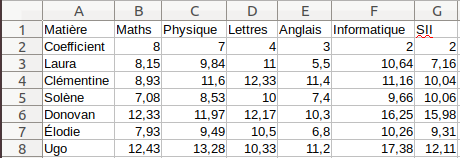
\includegraphics[width=10cm]{moyennes_matieres.png}
    \end{center}
    \caption{Tableau des moyennes de chaque étudiant, matière par matière.}
    \label{07:tab:moyennes_matieres}
\end{figure}

%\clearslide{}

En enregistrant ce ficher au format CSV (pour \emph{Comma-Separated Values}), on obtient le fichier \texttt{moyennes\_matieres.csv} suivant. 
\begin{lstlisting}
Matière;Maths;Physique;Lettres;Anglais;Informatique;SII
Coefficient;8;7;4;3;2;2
Laura;8,15;9,84;11;5,5;10,64;7,16
Clémentine;8,93;11,6;12,33;11,4;11,16;10,04
Solène;7,08;8,53;10;7,4;9,66;10,06
Donovan;12,33;11,97;12,17;10,3;16,25;15,98
Élodie;7,93;9,49;10,5;6,8;10,26;9,31
Ugo;12,43;13,28;10,33;11,2;17,38;12,11
\end{lstlisting}

%\clearslide{}

On peut commencer par extraire les données du tableau sous Python{} comme suit (la première ligne ne nous intéresse pas).

\begin{pyverbatim}
with open("moyennes_matieres.csv","r") as f : 
    _ = f.readline()
    coeffs = f.readline().strip().split(';')
    T = f.readlines()
\end{pyverbatim}
\begin{rem}
    Avec la méthode \pyv{strip}, on enlève directement le caractère \texttt{\textbackslash n} et les espaces éventuels à la fin de la ligne lue. 
\end{rem}

%\clearslide{}
On peut ensuite traiter la ligne des coefficients. 
\begin{pyverbatim}
n = len(coeffs)
S = 0 # Somme des coefficients
for i in range(1,n):
    coeffs[i] = int(coeffs[i])
    S = S + coeffs[i]
coeffs.append(S)
\end{pyverbatim}
\begin{rem}
    On a pris soin ici de convertir directement les coefficients dans le type adéquat et l'on a calculé la somme des coefficients, qui servira pour calculer la moyenne pondérée de chaque étudiant. 
\end{rem}
À la fin de ce traitement, voici l'état de la variable \pyv{coeffs}.
\begin{pyverbatim}
['Coefficient', 8, 7, 4, 3, 2, 2, 26]
\end{pyverbatim}

%\clearslide{}
On peut ensuite traiter le reste du tableau, comme suit. 
\begin{pyverbatim}
for i in range(len(T)) :
    T[i] = T[i].strip().split(';')
    for j in range(1,n):
        T[i][j] = float(T[i][j].replace(',','.'))
\end{pyverbatim}
\begin{rem}
    On a là encore pris soin d'enlever le caractère \texttt{\textbackslash n} à la fin de chaque ligne et de remplacer les \texttt{,} (notation décimale française) par des \texttt{.} (notation décimale anglaise). 
\end{rem}
À la fin de ce traitement, voici l'état de la variable \pyv{T}.
\begin{pyverbatim}
[['Laura', 8.15, 9.84, 11.0, 5.5, 10.64, 7.16], 
 ['Clémentine', 8.93, 11.6, 12.33, 11.4, 11.16, 10.04], 
 ['Solène', 7.08, 8.53, 10.0, 7.4, 9.66, 10.06], 
 ['Donovan', 12.33, 11.97, 12.17, 10.3, 16.25, 15.98], 
 ['Élodie', 7.93, 9.49, 10.5, 6.8, 10.26, 9.31], 
 ['Ugo', 12.43, 13.28, 10.33, 11.2, 17.38, 12.11]]
\end{pyverbatim}

%\clearslide{}
On peut ensuite calculer pour chaque étudiant sa moyenne pondérée comme suit. 
\begin{pyverbatim}
for e in T : 
    moy = 0
    for i in range(1,n):
        moy = moy + coeffs[i]*e[i]
    moy = moy / coeffs[-1]
    e.append(moy)
\end{pyverbatim}
À la fin de ce traitement, voici l'état de la variable \pyv{T}.
\begin{lstlisting}
[['Laura', 8.15, 9.84, 11.0, 5.5, 10.64, 7.16, 8.853076923076923], 
 ['Clémentine', 8.93, 11.6, 12.33, 11.4, 11.16, 10.04, 10.713846153846152], 
 ['Solène', 7.08, 8.53, 10.0, 7.4, 9.66, 10.06, 8.38423076923077], 
 ['Donovan', 12.33, 11.97, 12.17, 10.3, 16.25, 15.98, 12.55653846153846], 
 ['Élodie', 7.93, 9.49, 10.5, 6.8, 10.26, 9.31, 8.900384615384617], 
 ['Ugo', 12.43, 13.28, 10.33, 11.2, 17.38, 12.11, 12.549999999999999]]
\end{lstlisting}

%\clearslide{}
Il ne reste plus qu'à écrire les valeurs calculées dans un tableau, comme suit. 
\begin{pyverbatim}
with open("moyennes_ponderees.csv","w") as f : 
    f.write("Prénoms;Moyennes pondérées")
    for e in T : 
        f.write('\n'+';'.join([str(e[0]),str(e[-1])]))
\end{pyverbatim}
Le contenu du fichier \texttt{moyennes\_ponderees.csv} est le suivant. 
\begin{lstlisting}
Prénoms;Moyennes pondérées
Laura;8.853076923076923
Clémentine;10.713846153846152
Solène;8.38423076923077
Donovan;12.55653846153846
Élodie;8.900384615384617
Ugo;12.549999999999999
\end{lstlisting}
%\clearslide{}
Dans un tableur, on lit cela (voir figure~\ref{07:tab:moyennes_ponderees}).
\begin{figure}[h!]
    \begin{center}
        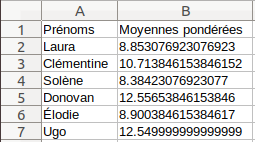
\includegraphics[width=6cm]{moyennes_ponderees.png}
    \end{center}
    \caption{Tableau des moyennes pondérées.}
    \label{07:tab:moyennes_ponderees}
\end{figure}

%\section{Exercices.}

%\begin{exo}
%  Vous trouverez sur le site de classe un fichier \texttt{cats.csv}.
Il contient des mesures de corpulence de chats. 
Vous y trouverez trois colonnes : le sexe de chaque chat (colonne \texttt{Sex}), son poids en kilogrammes (colonne \texttt{Bwt}) et le poids de son cœur en grammes (colonne \texttt{Hwt}). 

Écrire un script \python{} permettant de lire ce fichier et d'écrire dans un autre fichier, pour chaque sexe, le poids moyen et le poids du cœur moyen. 

%\end{exo}

%\begin{exo}
%  Écrire une fonction \texttt{moyennes(fichier\_notes,fichier\_moyennes,sep=',')} lisant les notes écrites dans \texttt{fichier\_notes} et écrivant dans le \texttt{fichier\_moyennes} le prénom de chaque élève, suivi par la moyenne de ses notes. 

Par convention, la première ligne de chaque fichier comporte les titres des colonnes et la première colonne contient le prénom de chaque étudiant. Un exemple (fichiers \texttt{notes.csv} et \texttt{moyennes.csv}) sera mis en ligne sur le site de classe. 

On respectera le format  \texttt{.csv}, le séparateur par défaut sera donc les virgules (\texttt{','}). 
%\end{exo}

%\begin{exo}
%  Vous trouverez sur le site de classe un fichier \texttt{sainte$\_$lyon.csv}.
Il contient la liste des 31 premiers concurrents de la course de trail nocture \textbf{La Saintélyon} de l'édition 2017 reliant Saint-Etienne à Lyon. 
Vous y trouverez deux colonnes : le nom de chaque concurrent (colonne \texttt{Nom}) et le temps mis pour parcourir le parcours de 72 km (colonne \texttt{Temps}) au format $heures:minutes:secondes$. 

\question{Écrire un script \python{} permettant de lire ce fichier et d'écrire dans un autre fichier, pour chaque nom, le temps en secondes et la vitesse en km/h.}

%\end{exo}


% \section*{Copyleft et crédits photographiques}
% \input{artlibre}
% 
% Photo de première page (serveurs de l'Internet Archive): \input{\titleimage.credits}
